\subsection{Sentences and punctuation statistics}

We then did some statistics on the sentences and the punctuation. We started by analysing the average length of the sentences (see figure  \ref{average_sent_length_figure}).

\begin{figure}[H]
	\centering
    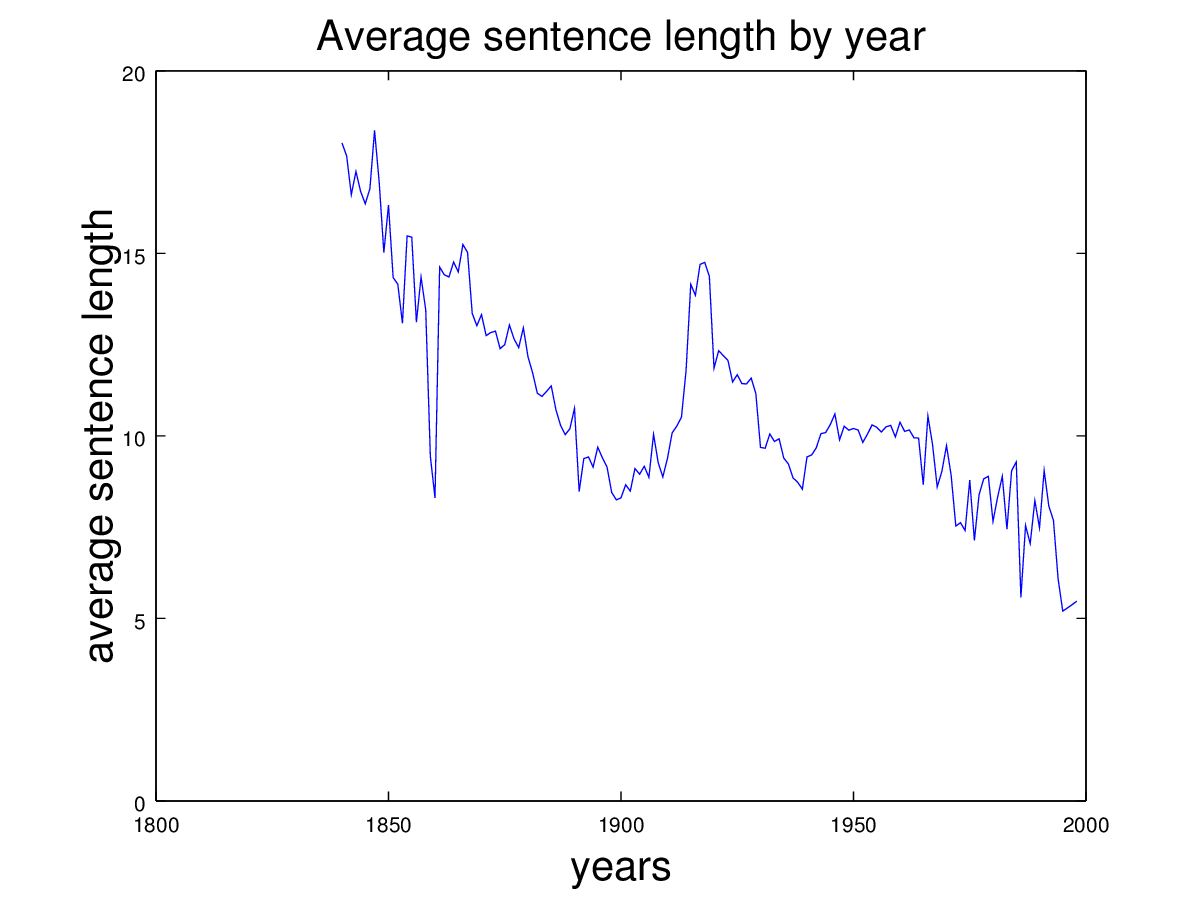
\includegraphics[scale=0.5]{Pictures/statistics/sentences-length/means.png}
    \caption{Average length of sentences by year}
    \label{average_sent_length_figure}\hfill
\end{figure}

\begin{figure}[H]
	\centering
    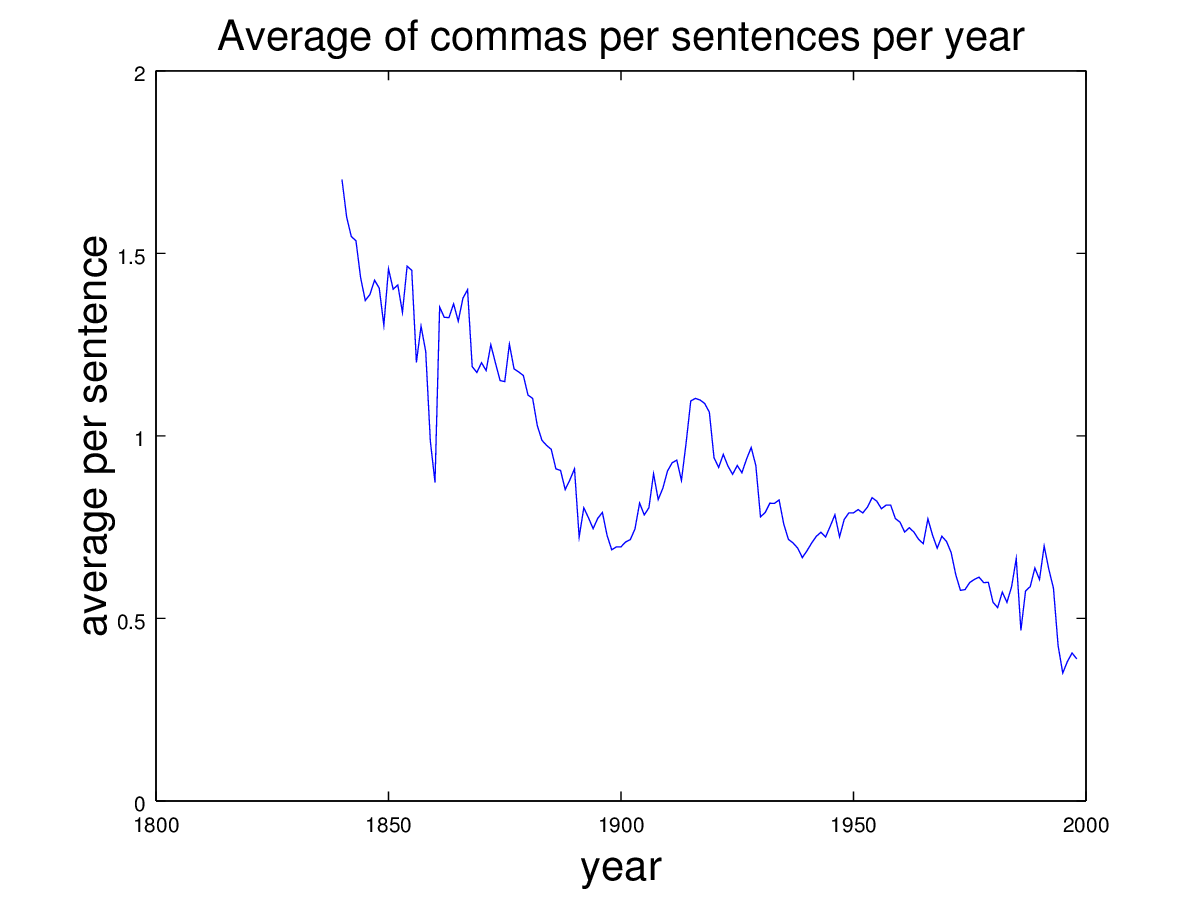
\includegraphics[scale=0.5]{Pictures/statistics/punctuation/graph.png}
    \caption{Average number of commas, semicolons and colons per sentence per year}
    \label{average_punct}\hfill
\end{figure}

If we ignore the down peak near 1850, oming from some unknown problem in two year (maybe less articles or big OCR problems) we see that the length of the sentences tends to decrease through time. In fact, the decrease is significant, going from 15-20 words by sentence in 1840 down to 8-10 words by sentence in 1990.

(Note : another problem apart from the bad OCR is that from year 1917 to 1919 (included), we were provided with only one of the two newspapers merging into "LeTemps" articles, what affects the statistics for those years as there are less articles than in the other years).

We can correlate those results with the statistics on punctuation. In figure \ref{average_punct}, the black curve represents the average of commas per sentences per year, the red curve the average of semicolons and the blue curve the average of colons. The two last curves are not really interesting in terms of linguistic drift as they do not vary much. In fact, the articles are using approximatly the same number of colons and semicolons from 1840 to 1990. The black curve however show that, there is a tendency to use less commas on articles, what is quite logical as sentences are shorter so we need to use less commas.\\

Again those statistics show the lignuistic drift, between 1840 and 1990 by showing the fact that, through time, shorter sentences are used in our corpus. This trivially affects the punctuation used. \\

As those observations shows a real variation between years, we thought it could be a good idea to use them for a metric. Results are presented in the next section.
